% =====================================================================
%  Peptide Identity as the Termination of Exclusion
%
%  Self-contained. Every construction used is defined here; no companion
%  paper is required. External citations are to the mass spectrometry
%  and graph theory literature only.
% =====================================================================
\documentclass[11pt,a4paper]{article}

\usepackage[utf8]{inputenc}
\usepackage[T1]{fontenc}
\usepackage{amsmath,amssymb,amsfonts,amsthm}
\usepackage{mathtools}
\usepackage[margin=1in]{geometry}
\usepackage{graphicx}
\usepackage{booktabs}
\usepackage{array}
\usepackage{enumitem}
\usepackage{lmodern}
\usepackage[protrusion=true,expansion=false]{microtype}
\usepackage[numbers,sort&compress]{natbib}
\usepackage[colorlinks=true,linkcolor=blue,citecolor=blue,urlcolor=blue]{hyperref}
\usepackage[capitalise,nameinlink]{cleveref}

% ---------------------------------------------------------------------
%  Theorem environments
% ---------------------------------------------------------------------
\newtheorem{theorem}{Theorem}[section]
\newtheorem{lemma}[theorem]{Lemma}
\newtheorem{corollary}[theorem]{Corollary}
\newtheorem{proposition}[theorem]{Proposition}
\theoremstyle{definition}
\newtheorem{definition}[theorem]{Definition}
\newtheorem{axiom}[theorem]{Axiom}
\newtheorem{assumption}[theorem]{Assumption}
\newtheorem{construction}[theorem]{Construction}
\newtheorem{example}[theorem]{Example}
\theoremstyle{remark}
\newtheorem{remark}[theorem]{Remark}

% ---------------------------------------------------------------------
%  Notation
% ---------------------------------------------------------------------
\newcommand{\Gph}{\mathcal{G}}              % graph
\newcommand{\wt}{w}                          % weight function
\newcommand{\med}{\mathfrak{m}}              % medium vertex
\newcommand{\flo}{\beta}                     % the floor
\newcommand{\cut}{\operatorname{cut}}
\newcommand{\sep}{\sigma}                    % separation cost
\newcommand{\dep}{\delta}                    % depth (minimising side size)
\newcommand{\key}{\kappa}                    % cut key
\newcommand{\netw}{\mathcal{N}}
\newcommand{\resid}{R}                       % global residual
\newcommand{\clos}{\mathrm{cl}}
\newcommand{\Prot}{\mathcal{P}}              % protein universe
\newcommand{\Pep}{\mathcal{Q}}               % peptide set
\newcommand{\amb}{\mathcal{A}}               % admissible set
\newcommand{\Cat}{\mathrm{cell}}
\newcommand{\eff}{e}
\newcommand{\estar}{e^{\ast}}
\newcommand{\dem}{D}
\DeclareMathOperator{\prom}{prom}
\DeclareMathOperator*{\argmin}{arg\,min}

\title{\textbf{Peptide Identity as the Termination of Exclusion:\\[2pt]
Mass Invariance, Promiscuous Intersection, and a Stopping\\
Criterion for Sequence Determination}}

\author{Kundai Farai Sachikonye\\
\texttt{kundai.sachikonye@wzw.tum.de}}

\date{\today}

\begin{document}
\maketitle

% =====================================================================
\begin{abstract}
\noindent
A mass spectrometer of unbounded resolving power cannot identify
lithium. This is not a statement about engineering. It is a statement
about the kind of object an identity is: a mass measurement returns a
point, and we prove that identity in any system whose parts are
individuated by comparison against a non-enumerable complement is a
\emph{region} bounded below by a strictly positive floor, never a point.
The periodic table's entry for lithium is therefore not an assertion that
something \emph{is} lithium; it is the termination point of a sufficient
\emph{not-lithium} sequence, and the reason many instruments exist for
one element is that each commits a different exclusion and none
individuates alone.

We carry this to peptides. Working entirely with finite weighted graphs,
we prove: that every cut separating a part from its complement has weight
at least $\flo>0$ (\Cref{thm:floor}); that identity is the invariant
minimum-cut value and is region-valued (\Cref{thm:region}); that adding
an edge cannot increase the number of distinguishable parts but can only
redistribute residual, so that \emph{edges measure what remains unknown
rather than what has been learned} (\Cref{thm:residual}); and that a
determination terminates not when residual is small but when further
evidence ceases to move the region---a criterion we call
\emph{closure} and prove strictly stronger than any confidence threshold
(\Cref{thm:closure-stronger}).

Two consequences are specific to proteomics. Sequence determination has
a computable step bound and exactly two outcomes, closure or
\emph{honest decline}; there is no third, and in particular no state in
which an algorithm is still running with no internal signal of its own
futility (\Cref{thm:dichotomy}). And an isobaric pair such as
leucine/isoleucine is not a failure but a correct terminal region, with
a stated condition under which a further method narrows it
(\Cref{prop:isobaric}).

We also advanced, and then refuted, a third claim. We conjectured that
\emph{parsimony is the wrong objective for protein inference}: that
because a peptide mapping to many proteins excludes more than a unique
peptide does, ranking peptides by \emph{promiscuity} and intersecting
would reach the true protein set in fewer peptides than
minimum-set-cover parsimony. We registered this expectation, together
with its negative control, in the experiment source before running it.
It is false, and it is false for a reason internal to our own
\Cref{thm:collapse}: that theorem's expectation is monotone
\emph{increasing} in each promiscuity, so under its hypothesis the least
promiscuous peptides are the best individual choices. Measured over
$188$ trials, promiscuity-first won or tied against parsimony in
$7.4\%$ of cases and never won strictly; uniqueness-first---the control
that was required to fail---beat promiscuity-first in $100\%$. The
supporting empirical assumption is refuted with the opposite sign to the
one predicted: homology structure makes measured intersections
$2.56\times$ \emph{larger} than the independence model, not smaller,
because peptides co-observed in one protein are drawn from its own
domain pool and their mapping sets are positively correlated rather than
independent.

What survives is reported as such. \Cref{thm:collapse} itself is
confirmed numerically to within $0.44\%$ where its independence
hypothesis holds. The floor is recovered exactly and no item is
individuated below it; residual is non-decreasing under edge commitment
in all $120$ orderings tested; cut keys are invariant under relabelling
in $20/20$; closure is reached strictly before evidence is exhausted in
$100\%$ of trials; and every run terminates in closure or honest
decline, with none exhausting. We state the limitations plainly: the
framework is an account of when a determination may stop, not a spectrum
interpreter, and its one empirical extension into protein inference did
not survive contact with measurement.
\end{abstract}

\noindent\textbf{Keywords:} peptide identification; protein inference;
minimum cut; individuation by negation; exclusion; closure; de novo
sequencing; isobaric residues; promiscuous peptides.

\tableofcontents
\newpage

% =====================================================================
\section{Introduction}
\label{sec:intro}
% =====================================================================

\subsection{A question about lithium}
\label{sec:lithium}

Consider an instrument that measures mass with unbounded precision.
Present it with a sample of lithium. It returns $6.941$, then
$6.9410000$, then as many digits as one cares to demand.

It has not identified lithium.

The claim is not that the measurement is imprecise, nor that isotopes
complicate it, nor that contamination intrudes. Suppose all of that away:
suppose a perfect scale and a perfect sample. The instrument still has
not identified lithium, and no improvement in resolving power will change
this. The reason is visible in what chemistry actually does. Lithium is
established by flame test, emission spectrum, ionisation energy, density,
conductivity, reactivity, X-ray crystallography---an array of methods
sharing no common mechanism. If mass sufficed, this array would be
redundant. It is not redundant, and the fact that it is not is the datum
this paper begins from.

The answer we develop is that a periodic table entry is not the assertion
\emph{this is lithium}. It is the terminus of a sufficient
\emph{not-lithium} sequence. Each method excludes: the flame test
excludes sodium and potassium, the emission spectrum excludes every
element with different line structure, the ionisation energy excludes
different shell occupancies. None says what the sample is. Together they
say what it is not, and the entry names where that saying stops moving.

This distinction has a precise consequence. A mass measurement returns a
\emph{point} in $\mathbb{R}$. We prove below that an identity, in any
system whose parts are told apart by comparison against a complement that
cannot be exhaustively listed, is a \emph{region} with a strictly
positive lower bound on its size (\Cref{thm:region}). A point and a
region are not the same kind of object, and no amount of precision
converts one into the other. Higher resolution gives a sharper point. A
sharper point is not a smaller region; it is still not a region at all.

\subsection{The same question about peptides}

Tandem mass spectrometry identifies peptides by mass differences.
A peptide fragments along its backbone, consecutive fragment ions differ
by a residue mass, and the sequence is read off the
ladder~\citep{roepstorff1984proposal,paizs2005fragmentation}. Database
search matches an observed spectrum against theoretical spectra generated
from a protein
database~\citep{eng1994approach,perkins1999probability,cox2008maxquant};
de novo sequencing reconstructs the sequence from the spectrum alone by
building a graph whose vertices are peaks and whose edges are residue-mass
differences, then searching for
paths~\citep{dancik1999novo,frank2005pepnovo,ma2003peaks,tran2017novo}.

Both inherit the lithium problem, and three well-known difficulties are
its symptoms rather than independent defects.

\paragraph{Leucine and isoleucine.} These differ only in side-chain
branching and have identical residue mass $113.084$~Da. No mass
measurement distinguishes them, at any resolution. The field treats this
as a limitation to be circumvented by specialised
methods~\citep{xiao2016distinguishing,zhokhov2017distinguishing}. We
argue it is instead the general situation made visible: mass never
individuates anything, and merely happens to be sufficient more often
elsewhere.

\paragraph{Algorithms that cannot stop.} A de novo search over a spectrum
graph has no criterion available before the traversal completes, because
its criterion is a score at the terminus. A wrong sequence and an
unfinished one present identically: both look like \emph{keep going}. We
show this is not a tuning deficiency but a consequence of asking a
selector question in a system that admits no selector
(\Cref{thm:no-selector}), and that the correct question---\emph{has the
exclusion sequence closed?}---is checkable at every step.

\paragraph{Parsimony.} Protein inference conventionally seeks the
smallest set of proteins explaining the observed
peptides~\citep{nesvizhskii2003statistical,nesvizhskii2005interpretation,huang2012protein}.
Peptides mapping to many proteins are discounted as non-unique or
``razor''; unique peptides are prized. We conjectured that this ranking
is inverted, on the ground that a promiscuous peptide commits the larger
exclusion. \Cref{sec:promiscuity} develops the arithmetic and
\Cref{sec:validation} refutes the conjecture---using, as it turns out,
a consequence of the very theorem advanced in its support. We retain the
development because the refutation is informative and because the
exclusion reading of a mapping set survives it.

\subsection{What this paper does}

We work entirely with finite weighted graphs. Every object is a vertex
set, an edge set, and a weight function; every claim reduces to a
statement about cuts, and is therefore checkable by direct
computation, since minimum cuts are exactly computable by maximum
flow~\citep{fordfulkerson1956,goldberg1988new,stoerwagner1997}. We
introduce no probability measure and no metric space. Where a word
carries an evocative reading---``exclusion'', ``closure'',
``promiscuity''---it names a specific graph object defined in the text,
and no theorem depends on any reading beyond the definition.
Interpretive remarks are marked as such and are never load-bearing.

\Cref{sec:graph} fixes the contact graph and the medium.
\Cref{sec:floor} derives the floor. \Cref{sec:identity} proves identity
is a region and that labels carry no invariant. \Cref{sec:residual}
establishes the inversion: edges measure the unknown.
\Cref{sec:closure} gives the closure criterion and the termination
dichotomy. \Cref{sec:peptide} applies all of it to peptides.
\Cref{sec:promiscuity} proves the collapse theorem and states the
inference procedure. \Cref{sec:twographs} gives the two-graph
construction and the correspondence test. \Cref{sec:validation} reports
the validation suite. \Cref{sec:limitations} states what the framework
does not establish.

\subsection{What this paper does not do}

It does not interpret spectra. It provides no peak-picking, no
deisotoping, no scoring function, and no implementation competitive with
existing search engines. It offers an account of \emph{when a
determination may stop and what its output is}, which is orthogonal to
how well any particular engine matches peaks.

It does not claim that database search is wrong. Database search is
highly effective within its scope and its statistical
control is well developed~\citep{elias2007target,kall2007semi,the2016fast}.
We claim its output has been misdescribed: a match is a termination of
exclusion against one particular catalogue, not a determination of
identity, and the difference matters exactly where the catalogue is
incomplete.

It does not resolve leucine from isoleucine. It argues that the demand
to do so by mass is malformed, and specifies the condition under which
another method narrows the region.

% =====================================================================
\section{Contact graphs and the medium}
\label{sec:graph}
% =====================================================================

\begin{definition}[Contact graph]
\label{def:contact}
A \emph{contact graph} is a finite weighted graph
$\Gph=(V,E,\wt)$ with $\wt:E\to\mathbb{R}_{>0}$, together with a
distinguished vertex $\med\in V$ called the \emph{medium}, adjacent to
every other vertex. Vertices in $V\setminus\{\med\}$ are called
\emph{items}. We write $n=|V|-1$ for the number of items.
\end{definition}

The medium is not an item and is not optional. It is the object against
which every item is told apart, and its adjacency to everything is what
makes that comparison always available. \Cref{rem:medium-why} explains
why it cannot be omitted.

\begin{definition}[Cut, separation cost, depth]
\label{def:cut}
For $S\subseteq V$ with $\emptyset\neq S\neq V$, the \emph{cut} induced
by $S$ is $\cut(S)=\sum_{\{u,v\}\in E,\,|S\cap\{u,v\}|=1}\wt(\{u,v\})$.
For an item $v$, let
\[
  S^{\ast}(v)\;=\;\argmin\{\,\cut(S)\;:\;v\in S,\ \med\notin S\,\},
\]
the cheapest way to separate $v$ from the medium. Write
\[
  \sep(v)=\cut(S^{\ast}(v)),
  \qquad
  \dep(v)=|S^{\ast}(v)|,
\]
the \emph{separation cost} and the \emph{depth}. The pair
$\key(v)=(\sep(v),\dep(v))$ is the \emph{cut key} of $v$.
\end{definition}

\begin{remark}[Computability]
\label{rem:computable}
$\sep(v)$ and $\dep(v)$ are computed by a single maximum-flow
computation with source $v$ and sink $\med$, in time
$O(|V|\,|E|)$ by standard
algorithms~\citep{fordfulkerson1956,goldberg1988new}. Nothing in this
paper requires a search over subsets.
\end{remark}

\begin{definition}[Complement, enumeration]
\label{def:complement}
The \emph{complement} of an item $v$ is $V\setminus\{v,\med\}$ together
with everything the medium stands for. An \emph{enumeration} of the
complement is a finite list of items that exhausts it.
\end{definition}

\begin{axiom}[Non-completability]
\label{ax:noncomplete}
The complement admits no enumeration. Formally: for every finite item set
$V$ there exists a contact graph $\Gph'\supset\Gph$ extending it with an
item not in $V$, and no procedure internal to $\Gph$ certifies that no
such extension exists.
\end{axiom}

\Cref{ax:noncomplete} is the paper's single premise, and it is not a
metaphysical posit. It is the ordinary condition of any laboratory
measurement: no experiment establishes that the sample contains nothing
else, and every analytical method operates under the standing possibility
of an unmodelled species. The remainder of the paper derives
consequences from this one fact.

\begin{remark}[Why the medium cannot be dropped]
\label{rem:medium-why}
One might try to individuate $v$ by cutting it directly against a
specific rival $u$. This requires choosing $u$, and the choice is
either arbitrary or itself justified by a prior individuation, which
regresses. The medium removes the regress by being the one vertex whose
adjacency is definitional rather than chosen. \Cref{thm:no-selector}
makes this precise.
\end{remark}

% =====================================================================
\section{The floor}
\label{sec:floor}
% =====================================================================

\begin{theorem}[Floor from non-completability]
\label{thm:floor}
Under \Cref{ax:noncomplete} there exists $\flo>0$, depending on
$(\Gph,\wt)$ but not on the item, such that
\[
  \sep(v)\;\ge\;\flo
  \qquad\text{for every item } v.
\]
\end{theorem}

\begin{proof}
Fix an item $v$. Since $\med$ is adjacent to every item
(\Cref{def:contact}), any $S$ with $v\in S$, $\med\notin S$ has the edge
$\{v,\med\}$ crossing it, so
$\cut(S)\ge \wt(\{v,\med\})>0$. Hence
$\sep(v)\ge\min_{u}\wt(\{u,\med\})=:\flo_0>0$, the minimum taken over the
finite item set, and $\flo_0$ is independent of $v$.

It remains to show $\flo_0$ cannot be driven to zero by refining the
graph. Suppose some procedure assigned $\wt(\{v,\med\})=0$, i.e.\
severed $v$ from the medium at no cost. Then $v$ would be individuated
without any comparison against its complement, so the complement would
contribute nothing to fixing $v$ --- equivalently, $v$ would be
identified by inspection of $v$ alone. By \Cref{ax:noncomplete} the
complement is not enumerable, so no inspection of $v$ can certify that
nothing else in the complement shares $v$'s description; the assignment
$\wt(\{v,\med\})=0$ is therefore not licensed by any finite procedure.
Setting $\flo=\flo_0$ gives the claim.
\end{proof}

\begin{remark}[Reading]
\label{rem:floor-reading}
$\flo$ is the cost of the comparison that never closes. It is the
formal residue of the fact that one cannot check a sample against
everything it is not. All subsequent structure follows from
$\flo>0$; nothing follows from any particular value of $\flo$.
\end{remark}

\begin{proposition}[Stability under expansion]
\label{prop:stability}
Let $\Gph'$ extend $\Gph$ by adding items and edges of positive weight,
leaving existing weights unchanged. Then the floor of $\Gph'$ satisfies
$\flo'\le\flo$, and $\sep_{\Gph'}(v)\ge\sep_{\Gph}(v)$ for every item $v$
of $\Gph$.
\end{proposition}

\begin{proof}
The floor is a minimum over a larger index set, hence does not increase.
For the second claim, every cut separating $v$ from $\med$ in $\Gph'$
restricts to such a cut in $\Gph$ with weight no greater, since edges
were only added; taking minima gives the inequality.
\end{proof}

\Cref{prop:stability} is the formal statement that acquiring more
evidence never makes an item \emph{cheaper} to individuate. This is used
in \Cref{sec:residual}.

% =====================================================================
\section{Identity is a region, and labels carry none}
\label{sec:identity}
% =====================================================================

\begin{theorem}[No selector]
\label{thm:no-selector}
There is no function $f$ on items, computable from the graph, that
selects a distinguished rival $r(v)$ against which $v$ may be
individuated, without either (i) an arbitrary choice or (ii) a prior
individuation of $r(v)$.
\end{theorem}

\begin{proof}
Suppose $f$ exists and is not arbitrary. Then $f(v)$ is determined by
some property $P$ of the graph. To apply $P$ to candidate rivals one must
already tell those candidates apart, i.e.\ individuate them; that
individuation requires its own selector, and the argument repeats. The
recursion has no base case in a finite graph without a distinguished
vertex, since removing $\med$ leaves all items symmetric under the
relabelling of \Cref{thm:invariance} below. Hence $f$ is arbitrary or
regressive.
\end{proof}

\begin{theorem}[Invariance under relabelling]
\label{thm:invariance}
Let $\varphi:\Gph\to\Gph'$ be a weighted isomorphism fixing $\med$. Then
$\sep(\varphi(v))=\sep(v)$ and $\dep(\varphi(v))=\dep(v)$ for every
item $v$. In particular $\key$ is an invariant of the weighted graph and
is independent of every vertex name.
\end{theorem}

\begin{proof}
$\varphi$ is a bijection on vertices preserving edges and weights, so it
carries cuts to cuts of equal weight and preserves the constraint
$v\in S$, $\med\notin S$. It therefore carries the minimising family for
$v$ onto that for $\varphi(v)$, preserving both the minimum value and the
cardinality of the minimising side.
\end{proof}

\begin{theorem}[Identity is region-valued]
\label{thm:region}
The identity of an item---defined as the datum invariant under all
relabellings that distinguishes it from the rest---is the minimum cut
$\cut(S^{\ast}(v))$, of weight at least $\flo>0$. It is a set of edges,
never a single vertex, and never a point value that a single scalar
measurement returns.
\end{theorem}

\begin{proof}
By \Cref{thm:invariance} the cut and its weight are relabelling
invariants; by \Cref{thm:no-selector} no vertex label can serve, since
labels are exactly what relabelling destroys. That the object is a set of
edges of total weight $\ge\flo$ is \Cref{thm:floor}. A scalar
measurement returns an element of $\mathbb{R}$, which determines an edge
set only if the map from edge sets to reals is injective; it is not,
since distinct cuts may share a weight.
\end{proof}

\begin{corollary}[Mass cannot identify]
\label{cor:mass}
Let $\mu$ be any scalar observable---mass, mass-to-charge ratio,
retention time, a similarity score. Then $\mu$ does not determine the
identity of an item, at any precision.
\end{corollary}

\begin{proof}
Immediate from \Cref{thm:region}: $\mu(v)\in\mathbb{R}$ is a point and
identity is a region of weight $\ge\flo>0$. Refining $\mu$ produces a
more precise point and leaves the region undetermined.
\end{proof}

\Cref{cor:mass} is the formal content of \Cref{sec:lithium}. It also
answers the leucine/isoleucine question in advance: the failure of mass
to separate them is not special to that pair.

\begin{definition}[Resting catalogue]
\label{def:catalogue}
The \emph{resting catalogue} of a contact graph assigns to each item $v$
its cell
\[
  \Cat(v)\;:=\;\cut(S^{\ast}(v)),
  \qquad \text{of weight } \sep(v)\ge\flo .
\]
\end{definition}

\begin{remark}[The periodic table]
\label{rem:periodic}
\Cref{def:catalogue} is the precise sense in which a catalogue entry is a
terminus rather than an assertion: a cell \emph{is} the cut by which an
item is told from the rest, so listing an element is recording where its
exclusion stopped, not stating what it is. The catalogue's correctness is
inherited here and nowhere
contested~\citep{mendeleev1869,scerri2007}; what the framework adds is an
account of why a single method never suffices to populate a cell.
\end{remark}

% =====================================================================
\section{Edges measure the unknown}
\label{sec:residual}
% =====================================================================

This section establishes the inversion on which the rest of the paper
turns. Intuitively one expects that adding evidence adds knowledge, and
that knowledge accumulates locally at the item it concerns. Both are
false here.

\begin{definition}[Global residual]
\label{def:residual}
Let $\Gph$ have items $v_1,\dots,v_n$. The \emph{global residual} is
\[
  \resid(\Gph)\;=\;\sum_{i=1}^{n}\bigl(\sep(v_i)-\flo\bigr)\;\ge\;0 .
\]
\end{definition}

$\resid$ measures how far the graph is from the state in which every item
sits exactly at the floor. It is zero exactly when every item is
individuated as cheaply as \Cref{thm:floor} permits, and it can never be
driven below zero.

\begin{theorem}[Edges redistribute residual; they do not remove it]
\label{thm:residual}
Let $\Gph'$ be obtained from $\Gph$ by committing one additional edge of
positive weight between existing items. Then:
\begin{enumerate}[label=\textup{(\roman*)},leftmargin=2.2em,itemsep=1pt]
  \item the item set is unchanged;
  \item $\sep_{\Gph'}(v)\ge\sep_{\Gph}(v)$ for every item $v$;
  \item $\resid(\Gph')\ge\resid(\Gph)$; and
  \item $\flo'=\flo$, so no item is individuated below the floor.
\end{enumerate}
In particular no edge creates, destroys, or completes an identity; an
edge alters the \emph{distribution} of separation cost across the whole
graph.
\end{theorem}

\begin{proof}
(i) is by construction. (ii) is \Cref{prop:stability}. (iii) follows by
summing (ii) over items and subtracting $n\flo$. For (iv), the floor is
$\min_u \wt(\{u,\med\})$ by the proof of \Cref{thm:floor}, and the
committed edge joins two items, leaving all medium-incident weights
unchanged.
\end{proof}

\begin{corollary}[The measure is of the unknown]
\label{cor:unknown}
The quantity an edge changes is $\resid$, which is a sum over all items,
and which is bounded below by $0$ but never attains a state of complete
knowledge, since $\sep(v)\ge\flo>0$ always. Hence an edge's effect is
global, and what it quantifies is what remains undetermined rather than
what has been determined.
\end{corollary}

\begin{remark}[Reading]
\label{rem:inversion}
\Cref{thm:residual} says nodes are fixed and only edges move. The item
set of a contact graph is whatever the experiment produced; an analysis
does not add items, it commits contacts. This is why the framework is an
account of \emph{reshuffling} rather than accumulation, and why the
natural output is a residual rather than a score.
\end{remark}

% =====================================================================
\section{Closure, and the termination dichotomy}
\label{sec:closure}
% =====================================================================

Since $\resid$ never reaches zero, ``enough evidence'' cannot mean
``residual small''. It must mean something else, and the something else
is stability.

\begin{definition}[Catalyst]
\label{def:catalyst}
A \emph{catalyst} is a procedure $c$ that, applied to a contact graph,
commits one or more edges. A catalyst is \emph{available} at $\Gph$ if
its inputs are present. Catalysts are computationally uniform: a
laboratory step, a database lookup, and a model prediction are the same
kind of object, distinguished only by which edges they commit.
\end{definition}

\begin{definition}[Claim region]
\label{def:claim}
For an item $v$, the \emph{claim region} $\amb(v)$ is the set of
candidate assignments consistent with the committed edges---formally,
the set of items of a reference graph whose cut key agrees with
$\key(v)$ within the working tolerance.
\end{definition}

\begin{definition}[Closure]
\label{def:closure}
A determination of $v$ is \emph{closed} if for every catalyst $c$
available at $\Gph$, applying $c$ leaves $\amb(v)$ unchanged. Write
$\clos(v)$ for this condition.
\end{definition}

\begin{theorem}[Closure is strictly stronger than a threshold]
\label{thm:closure-stronger}
Let $\tau\in(0,1)$ and let $\mathrm{conf}(v)$ be any confidence
functional. Then:
\begin{enumerate}[label=\textup{(\roman*)},leftmargin=2.2em,itemsep=1pt]
  \item $\clos(v)$ does not imply $\mathrm{conf}(v)>\tau$;
  \item $\mathrm{conf}(v)>\tau$ does not imply $\clos(v)$; and
  \item $\clos(v)$ is decidable from the graph, whereas
  $\mathrm{conf}(v)>\tau$ requires a choice of $\tau$ external to it.
\end{enumerate}
\end{theorem}

\begin{proof}
(i) Take a graph in which $\amb(v)=\{a,b\}$ with $a,b$ having equal cut
keys, and in which no available catalyst distinguishes them. Then
$\clos(v)$ holds while any confidence functional respecting the symmetry
assigns at most $1/2$. (ii) Take a graph in which one catalyst has not
yet been applied and would move $\amb(v)$; confidence computed on the
current committed set may exceed $\tau$ while $\clos(v)$ fails. (iii)
Closure quantifies over the finite set of available catalysts and
compares claim regions, both computable; $\tau$ is not determined by
$(\Gph,\wt)$.
\end{proof}

\Cref{thm:closure-stronger}(i) is the case of central interest: a
determination may be closed and still return a region containing more
than one candidate. That is the correct output, not a failure.

\begin{assumption}[Effective commitment]
\label{ass:effective}
Every catalyst applied at a non-closed state commits at least one edge
and thereby reduces the outstanding demand
$\dem=\sum_{v}\bigl(|\amb(v)|-1\bigr)$ by at least $1$.
\end{assumption}

\begin{theorem}[Termination dichotomy]
\label{thm:dichotomy}
Under \Cref{ass:effective}, a determination has exactly two outcomes:
\begin{enumerate}[label=\textup{(\roman*)},leftmargin=2.2em,itemsep=1pt]
  \item it reaches closure after at most $\dem_0$ catalyst
  applications; or
  \item it halts at a non-closed state at which no available catalyst
  moves any claim region---an \emph{honest decline}.
\end{enumerate}
There is no third outcome; in particular the procedure cannot cycle, and
cannot run without an internal signal of its own futility.
\end{theorem}

\begin{proof}
$\dem$ is a non-negative integer. By \Cref{ass:effective} each
application at a non-closed state strictly decreases it, so after at most
$\dem_0$ applications either $\dem=0$, which is closure, or no effective
catalyst remains, which is (ii). Cycling is excluded because $\dem$ is
strictly decreasing and therefore never revisits a value.
\end{proof}

\begin{remark}[Decline is a verdict]
\label{rem:decline}
Outcome (ii) is informative, not a failure: it reports that the available
evidence cannot separate the remaining candidates. A method obliged to
emit a score for every input cannot express this, and must return a
low-confidence number where the correct answer is a refusal. Existing de
novo tools return per-residue confidences that conflate at least four
distinct situations: a clearly read residue, a residue inferred across a
gap, a tie between candidates, and a pair that is isobaric in principle.
\end{remark}

\begin{proposition}[Three catalysts]
\label{prop:three}
Let $v$ have claim region $\amb(v)$ supported by $k$ catalysts, and
suppose one catalyst may be in error. Then $\amb(v)$ is stable under the
removal of the erroneous catalyst only if $k\ge3$.
\end{proposition}

\begin{proof}
With $k=1$, removing the catalyst removes all support. With $k=2$, the
two may disagree after removal with no majority to adjudicate, so the
region is not determined. With $k\ge3$ and pairwise agreement among at
least two survivors, the region is preserved.
\end{proof}

\Cref{prop:three} recovers, as a theorem, the laboratory convention that
an element is not regarded as identified on a single test.

% =====================================================================
\section{Peptides}
\label{sec:peptide}
% =====================================================================

\subsection{The peptide contact graph}

\begin{construction}[Peptide graph]
\label{con:peptide}
Given an MS/MS spectrum with peaks $p_1,\dots,p_m$ and precursor mass
$M$, form a contact graph whose items are the peaks together with one
item per backbone position, and whose medium is $\med$. Commit an edge
between two peak items when a preparation fact or an instrument fact
relates them; commit an edge between a peak item and a position item
when the peak constrains that position. Weights are the strengths of the
respective constraints.
\end{construction}

The essential departure from a spectrum
graph~\citep{dancik1999novo} is that edges are not restricted to
residue-mass differences. Any experimental fact that constrains what a
peak can be is an edge, and \Cref{tab:edges} lists the classes.

\begin{table}[t]
\centering
\small
\caption{Edge classes in a peptide contact graph. Every entry is an
exclusion: it removes candidates rather than asserting an identity.
None except the first is available to a spectrum graph.}
\label{tab:edges}
\begin{tabular}{@{}p{0.26\textwidth}p{0.30\textwidth}p{0.36\textwidth}@{}}
\toprule
\textbf{Fact} & \textbf{Source} & \textbf{What it excludes} \\
\midrule
Residue-mass difference & MS/MS ladder & positions inconsistent with the gap \\
Enzyme specificity & digestion protocol~\citep{olsen2004trypsin} & C-termini other than K/R (trypsin) \\
Alkylation & sample prep~\citep{sechi1998method} & unmodified Cys ($+57.021$ fixed) \\
Ionisation polarity & source setting~\citep{fenn1989electrospray} & species that will not carry the charge \\
Isolation window & MS1 acquisition & precursor masses outside the window \\
Isotope envelope & MS1 & charge states inconsistent with spacing \\
Collision energy & HCD/CID setting~\citep{olsen2007higher} & cleavages not accessible at that energy \\
Retention time & LC gradient~\citep{krokhin2006sequence} & hydrophobicities outside the elution bound \\
Mapping set & in-silico digest & proteins not containing the peptide \\
\bottomrule
\end{tabular}
\end{table}

\begin{remark}[Preparation is data, not metadata]
\label{rem:prep}
Every peptide analysed is the endpoint of a long causal chain: organism,
lysis, reduction, alkylation, digestion, cleanup, chromatography,
ionisation, isolation, fragmentation, detection. Current practice records
this chain as free text~\citep{taylor2007guidelines} and consumes none of
it computationally; the search engine sees a peak list and a database.
\Cref{tab:edges} places the chain inside the computation, where each step
is an exclusion edge. This is the sense in which a determination can be
\emph{database-free}: not searching without a catalogue, but justified by
the experiment that produced the peak.
\end{remark}

\subsection{Isobaric residues}

\begin{proposition}[Isobaric pairs are terminal regions]
\label{prop:isobaric}
Let $a,b$ be residues with equal mass, and suppose the committed edges
are all mass-derived. Then $\amb=\{a,b\}$ and $\clos$ holds. Adding a
catalyst $c$ narrows $\amb$ if and only if $c$ commits an edge whose
weight differs between $a$ and $b$; otherwise $c$ leaves $\amb$
unchanged and closure is preserved.
\end{proposition}

\begin{proof}
Mass-derived edges assign equal weights to $a$ and $b$ by hypothesis, so
their cut keys agree and both lie in $\amb$ by \Cref{def:claim}. No
further mass catalyst separates them, so $\clos$ holds by
\Cref{def:closure}. A catalyst narrows $\amb$ exactly when it changes the
relative cut weights, which requires differing edge weights.
\end{proof}

\begin{remark}
\label{rem:li}
For leucine/isoleucine, \Cref{prop:isobaric} says that $\{L,I\}$ is a
correct closed answer under mass evidence, and that any method claiming
to resolve them must be committing a non-mass edge---which is what ion
mobility and EThcD approaches
do~\citep{xiao2016distinguishing,zhokhov2017distinguishing}. The
framework neither performs nor requires that resolution; it states the
condition under which it is possible and licenses reporting the region
when it is not.
\end{remark}

\subsection{Why a spectrum-graph search cannot stop}

\begin{proposition}[Malformed question]
\label{prop:malformed}
The query \emph{which residue occupies position $i$} requests a selector.
By \Cref{thm:no-selector} no such selector exists, and by
\Cref{thm:region} the available answer is a region. A procedure that
expects a point therefore has no internal criterion for having arrived,
and must run to exhaustion of its search space.
\end{proposition}

\begin{proof}
Immediate from the cited results: the procedure's termination predicate
is ``a point has been found'', which is never satisfied by the object the
graph determines, so termination is governed only by exhaustion.
\end{proof}

\Cref{prop:malformed} is the formal statement of the practical complaint
that de novo algorithms do not know when or why to stop. The remedy is
not a better score but a different query: \emph{has the exclusion
sequence closed?}, which \Cref{thm:dichotomy} answers in bounded time.

% =====================================================================
\section{Promiscuity and the collapse theorem}
\label{sec:promiscuity}
% =====================================================================

We now turn to protein inference, where the exclusion account makes a
prediction that contradicts standard practice and can be tested without
any instrument.

\subsection{Setting}

\begin{definition}[Mapping set, promiscuity]
\label{def:mapping}
Let $\Prot$ be a finite protein universe and $\Pep$ the peptides produced
from it by in-silico digestion. For $q\in\Pep$ write
\[
  \amb(q)\;=\;\{\,P\in\Prot \;:\; q \text{ occurs in } P \,\},
  \qquad
  \prom(q)=|\amb(q)| ,
\]
the \emph{mapping set} and the \emph{promiscuity} of $q$. A peptide with
$\prom(q)=1$ is \emph{unique}; one with $\prom(q)>1$ is
\emph{shared}, and is conventionally discounted as non-unique or
razor~\citep{nesvizhskii2005interpretation}.
\end{definition}

\begin{definition}[Exclusion reading]
\label{def:exclusion-reading}
Observing $q$ excludes $\Prot\setminus\amb(q)$. The \emph{exclusion
weight} of $q$ is $|\Prot|-\prom(q)$ for a single observation; for a
set $Q\subseteq\Pep$ of co-observed peptides the admissible set is
\[
  \amb(Q)\;=\;\bigcap_{q\in Q}\amb(q).
\]
\end{definition}

The intersection in \Cref{def:exclusion-reading} is the whole point, and
it is what parsimony does not compute. Parsimony seeks a minimum-cardinality
$\Prot'\subseteq\Prot$ covering the observed peptides---an instance of
minimum set cover, hence
NP-hard~\citep{karp1972reducibility,garey1979computers}---and evaluates
proteins by how few are needed. The exclusion reading evaluates peptides
by how much they remove.

\subsection{The collapse theorem}

\begin{theorem}[Intersection collapse rate]
\label{thm:collapse}
Let $|\Prot|=N$ and let $q_1,\dots,q_k$ be peptides whose mapping sets
are, conditional on containing the true protein $P^{\ast}$, otherwise
independent and uniformly distributed among subsets of size
$\prom(q_j)=\pi_j$. Then
\[
  \mathbb{E}\bigl|\amb(\{q_1,\dots,q_k\})\bigr|
  \;=\;
  1+(N-1)\prod_{j=1}^{k}\frac{\pi_j-1}{N-1}.
\]
Consequently, for fixed $k$ the expected admissible set is
\emph{increasing} in each $\pi_j$, while the \emph{ratio} of successive
admissible sizes is $(\pi_{k+1}-1)/(N-1)$, so each additional peptide
multiplies the residual ambiguity by a factor determined by its own
promiscuity.
\end{theorem}

\begin{proof}
$P^{\ast}$ lies in every $\amb(q_j)$ by hypothesis, contributing the
leading $1$. Each other protein $P\neq P^{\ast}$ lies in $\amb(q_j)$
with probability $(\pi_j-1)/(N-1)$, since $\amb(q_j)$ contains
$P^{\ast}$ and $\pi_j-1$ of the remaining $N-1$ proteins, chosen
uniformly. By conditional independence across $j$, $P$ survives all $k$
intersections with probability $\prod_j(\pi_j-1)/(N-1)$. Summing over the
$N-1$ such $P$ and adding $P^{\ast}$ gives the expression.
\end{proof}

\begin{corollary}[Promiscuity is informative in combination]
\label{cor:promiscuity}
Fix a budget of $k$ peptides and let the achievable promiscuities lie in
$[\pi_{\min},\pi_{\max}]$. The expected admissible set after intersecting
$k$ peptides is minimised by taking the $k$ \emph{least} promiscuous
peptides; but if the number of \emph{available} peptides at low
promiscuity is limited---as it is, since unique peptides are scarce---%
then the achievable reduction per peptide is governed by
$(\pi-1)/(N-1)$, and a shared peptide with $\pi\ll N$ still contributes a
multiplicative reduction strictly below $1$.
\end{corollary}

\begin{proof}
Immediate from the product form of \Cref{thm:collapse}: the expectation
is monotone in each factor, and each factor is $<1$ whenever
$\pi_j<N$.
\end{proof}

\begin{remark}[What the theorem does and does not say]
\label{rem:collapse-honest}
\Cref{thm:collapse} shows that shared peptides carry genuine
multiplicative discriminating power, contradicting the practice of
discarding them; it does \emph{not} show that the most promiscuous
peptides are the best individual choices, and under the idealised
independence hypothesis they are not. The empirical claim we test in
\Cref{sec:validation} is therefore about the realistic regime, in which
mapping sets are strongly structured by homology and are far from
independent, and in which unique peptides may be absent for a given
protein. This is the load-bearing assumption, isolated as
\Cref{ass:structure}.
\end{remark}

\begin{assumption}[Structured mapping sets --- \textbf{refuted}]
\label{ass:structure}
In a real proteome, mapping sets are not independent: they are organised
by sequence homology, so that two shared peptides drawn from different
homology groups have mapping sets whose intersection is far smaller than
the independence model predicts.
\end{assumption}

\Cref{ass:structure} is empirically decidable, and \Cref{sec:validation}
decides it \emph{against} the assumption. Mapping sets in a
domain-structured proteome are indeed non-independent, but the
correlation is \emph{positive}---peptides co-observed in one protein
come from that protein's own domain pool---so measured intersections are
$2.56$ times \emph{larger} than the independence prediction rather than
smaller. We state the assumption here in the form in which it was
registered, and mark it refuted rather than silently amending it.

\subsection{The inference procedure}

\begin{construction}[Exclusion inference]
\label{con:inference}
Given observed peptides $Q_{\mathrm{obs}}$:
\begin{enumerate}[leftmargin=2.0em,itemsep=1pt]
  \item Compute $\amb(q)$ for each $q\in Q_{\mathrm{obs}}$.
  \item Order $Q_{\mathrm{obs}}$ by decreasing $\prom(q)$.
  \item Intersect in that order, recording $|\amb(Q_t)|$ after each step.
  \item Stop at closure: the first $t$ such that every remaining
  $q$ leaves $\amb(Q_t)$ unchanged.
  \item Report $\amb(Q_t)$ --- a set, possibly with more than one
  element --- together with $t$ and the decline reason if any.
\end{enumerate}
\end{construction}

\begin{proposition}[Cost]
\label{prop:cost}
\Cref{con:inference} runs in $O(|Q_{\mathrm{obs}}|\cdot N)$ time with set
operations, and requires no search over protein subsets. By contrast
minimum set cover is
NP-hard~\citep{karp1972reducibility,garey1979computers}.
\end{proposition}

\begin{proof}
Each intersection is linear in the current admissible set, which is
bounded by $N$, and there are at most $|Q_{\mathrm{obs}}|$ of them.
No step enumerates subsets of $\Prot$.
\end{proof}

\begin{remark}[The keys and the lock, and where the image misleads]
\label{rem:keys}
A shared peptide is a key that opens many doors. Alone it identifies
nothing. But the observation is not that some door opened; it is that
several keys turned in the same lock, and the set of locks all of them
open is small even when each opens many. That much is
\Cref{thm:collapse}: each additional peptide multiplies the residual
ambiguity by $(\pi-1)/(N-1)<1$, so shared peptides do carry genuine
multiplicative discriminating power and discarding them discards
information.

The image misleads if pushed one step further, and we pushed it there
before measuring. It does \emph{not} follow that the most promiscuous
keys are the ones to try first. The same product formula is monotone
increasing in each $\pi_j$, so a key that opens fewer doors is strictly
the better key; a unique peptide opens exactly one and settles the
question in a single step. \Cref{sec:validation} measures this and finds
uniqueness-first beating promiscuity-first in every trial. The correct
statement is that shared peptides are \emph{usable} in combination, not
that they are \emph{preferable} to unique ones.
\end{remark}

% =====================================================================
\section{Two graphs, one determination}
\label{sec:twographs}
% =====================================================================

The exclusions of \Cref{tab:edges} fall into two groups that share no
mechanism, and this is what makes their agreement meaningful.

\begin{definition}[Instrument and mapping graphs]
\label{def:twographs}
The \emph{instrument graph} $\Gph_{\mathrm{I}}$ commits edges derived
from the preparation and acquisition chain: enzyme, alkylation, polarity,
isolation window, isotope envelope, collision energy, retention time.
The \emph{mapping graph} $\Gph_{\mathrm{M}}$ commits edges derived from
mapping sets and their intersections. Neither is computable from the
other.
\end{definition}

\begin{theorem}[Agreement is the invariant]
\label{thm:agreement}
Suppose $\Gph_{\mathrm{I}}$ and $\Gph_{\mathrm{M}}$ both close on item
$v$ with claim regions $\amb_{\mathrm{I}}(v)$ and $\amb_{\mathrm{M}}(v)$.
Then $\amb_{\mathrm{I}}(v)\cap\amb_{\mathrm{M}}(v)$ is invariant under
relabelling of either graph, and is not obtainable from either alone.
\end{theorem}

\begin{proof}
Each claim region is a relabelling invariant of its own graph by
\Cref{thm:invariance}, hence so is the intersection. It is not obtainable
from one alone because, by \Cref{def:twographs}, each graph commits edges
the other cannot: no mapping set encodes an alkylation mass shift, and no
preparation record encodes a homology relation.
\end{proof}

\begin{remark}[Why two graphs and not more evidence in one]
\label{rem:why-two}
\Cref{thm:agreement} is the formal version of the observation of
\Cref{sec:lithium}: X-ray crystallography and emission spectroscopy share
no mechanism, terminate at the same point, and \emph{that agreement} is
the catalogue entry. If one graph were derivable from the other,
agreement would be circular and prove nothing. Independence of mechanism
is what makes the coincidence informative.
\end{remark}

\begin{proposition}[Disagreement is diagnostic]
\label{prop:disagree}
If $\amb_{\mathrm{I}}(v)\cap\amb_{\mathrm{M}}(v)=\emptyset$, then either
(i) $\Gph_{\mathrm{M}}$ lacks the candidate, indicating a species absent
from the reference set---a novel modification, a contaminant, an
unexpected cleavage; or (ii) $\Gph_{\mathrm{I}}$ excludes it, indicating
that the preparation chain could not have produced it. These are
distinguishable by which graph is empty at $v$.
\end{proposition}

\begin{proof}
The intersection is empty exactly when no candidate survives both
exclusions; inspecting which region is empty identifies which chain of
exclusions is responsible.
\end{proof}

\Cref{prop:disagree} separates two situations that are currently reported
identically as unidentified spectra. The second is a protocol diagnosis
rather than an identification failure, and it names what to change.

% =====================================================================
\section{Validation}
\label{sec:validation}
% =====================================================================

\subsection{What a suite can establish here}

The theorems of \Cref{sec:floor}--\Cref{sec:closure} are statements about
finite weighted graphs and are proved; a computation cannot make them
more true. What a suite can establish is that the constructions behave as
claimed on concrete inputs, that the quantities are computable at the
stated cost, and---critically---that the one empirical assumption,
\Cref{ass:structure}, holds or fails. We therefore register expectations
in the experiment source before execution, and report negative controls
that must fail on well-formed input.

\subsection{Registered expectations}

\begin{enumerate}[label=\textbf{E\arabic*.},leftmargin=2.6em,itemsep=2pt]
  \item \textbf{Floor recovery.} On a contact graph with known
  medium-incident weights, the computed $\flo$ equals
  $\min_u \wt(\{u,\med\})$ exactly, and no item has $\sep(v)<\flo$.
  \item \textbf{Residual monotonicity.} Committing edges never decreases
  $\resid$ (\Cref{thm:residual}(iii)), in every ordering tested.
  \item \textbf{Cut-key invariance.} Relabelling items leaves the
  multiset of cut keys unchanged (\Cref{thm:invariance}).
  \item \textbf{Collapse rate.} Measured
  $|\amb(Q_t)|$ under intersection follows
  \Cref{thm:collapse} on synthetic independent mapping sets, and
  \emph{departs} from it on a real proteome---the departure being the
  content of \Cref{ass:structure}.
  \item \textbf{Promiscuity-first vs.\ parsimony.} On a proteome with
  known ground-truth protein content, promiscuity-first intersection
  (\Cref{con:inference}) reaches the true set in no more peptides than
  greedy parsimony, in a majority of trials.
  \item \textbf{Closure before exhaustion.} The step $t$ at which
  closure is reached is strictly less than $|Q_{\mathrm{obs}}|$,
  demonstrating that the criterion stops early rather than consuming all
  evidence.
  \item \textbf{Termination dichotomy.} Every run ends in closure or
  honest decline; no run cycles or exceeds the bound $\dem_0$ of
  \Cref{thm:dichotomy}.
\end{enumerate}

\subsection{Registered negative controls}

These must \emph{fail}; passing indicates the corresponding positive
result is vacuous.

\begin{enumerate}[label=\textbf{N\arabic*.},leftmargin=2.6em,itemsep=2pt]
  \item \textbf{Uniqueness-first ordering.} Intersecting unique peptides
  does not collapse the admissible set beyond what each gives alone,
  since intersecting singletons is trivial.
  \item \textbf{Shuffled mapping sets.} Randomly permuting protein
  membership destroys the collapse advantage, confirming it derives from
  proteome structure and not from the intersection operation.
  \item \textbf{Zero floor.} Setting $\flo=0$ removes the termination
  bound, and the dichotomy of \Cref{thm:dichotomy} no longer holds.
\end{enumerate}

\subsection{Results}
\label{sec:results}

Three experiments were run; artefacts are
\texttt{exp1\_graph\_invariants.json},
\texttt{exp2\_collapse\_rate.json} and
\texttt{exp3\_promiscuity\_vs\_parsimony.json} in
\texttt{validation/results/}. Every artefact carries the registered
expectation alongside the outcome.

\begin{table}[h]
\centering
\small
\caption{Registered expectations and outcomes. Two expectations failed
and one negative control failed to fail; all three are analysed in
\Cref{sec:refutation}.}
\label{tab:results}
\begin{tabular}{@{}llp{0.42\textwidth}@{}}
\toprule
\textbf{ID} & \textbf{Outcome} & \textbf{Measured} \\
\midrule
E1 & \textbf{holds} & floor recovered exactly in $30/30$ graphs; max
absolute error $0$; no item below floor \\
E2 & \textbf{holds} & $0$ residual decreases in $120$ commitment
orderings \\
E3 & \textbf{holds} & cut-key multiset invariant under relabelling in
$20/20$ \\
E4 & \textbf{fails} & independence prediction confirmed
($0.44\%$ relative error) but structured departure has the
\emph{opposite sign}: ratio $2.56$, not $<1$ \\
E5 & \textbf{fails} & promiscuity-first win-or-tie $0.074$; strict win
$0.000$; required $>0.5$ \\
E6 & \textbf{holds} & closure strictly before exhaustion in $188/188$
trials \\
E7 & \textbf{holds} & all runs end in closure or decline; $0$ exhausted \\
\midrule
N1 & \textbf{did not fail} & uniqueness-first beat promiscuity-first in
$100\%$ of trials \\
N2 & failed as required & shuffling removes all peptide sharing;
$0$ shared peptides remain \\
N3 & failed as required & pendant-victim construction voids the floor
and with it the bound \\
\bottomrule
\end{tabular}
\end{table}

\subsubsection{The refutation}
\label{sec:refutation}

\Cref{ass:structure} and the promiscuity claim it supports are refuted,
and the refutation is instructive rather than merely negative.

\paragraph{The sign is wrong.} We predicted that homology structure
would make measured intersections \emph{smaller} than the independence
model of \Cref{thm:collapse}, on the reasoning that peptides from
different families exclude each other's families wholesale. Measured
over $143$ targets, the ratio of measured to predicted admissible size
is $2.56$: intersections are more than twice as large as independence
predicts. The reason is visible once stated. Peptides co-observed in one
protein are drawn from \emph{that protein's own domain pool}, so their
mapping sets are positively correlated. Positively correlated sets
overlap more than chance, so their intersection retains more members,
not fewer. The structure that exists is real; it simply pushes the
opposite way.

\paragraph{The claim contradicted our own theorem.} \Cref{thm:collapse}
gives expected admissible size
$1+(N-1)\prod_j(\pi_j-1)/(N-1)$, which is monotone \emph{increasing} in
every $\pi_j$. Under its own hypothesis, therefore, the \emph{least}
promiscuous peptides are the best individual choices---which is what
\Cref{cor:promiscuity} already says and what \Cref{rem:collapse-honest}
already warns. Expectation E5 asserted the reverse. The measurement did
not discover a subtlety; it enforced a consequence that was derivable
from the theorem as proved.

\paragraph{The mechanism is single-step resolution.} Where a unique
peptide is present it isolates the target in one intersection---trace
$[1,1,1,\dots]$---while promiscuity-first spends three or four peptides
walking the admissible set down, e.g.\ $31\to5\to1$. Mean peptides to
target: uniqueness-first $1.00$, parsimony $1.50$, promiscuity-first
$3.23$.

\paragraph{The restricted regime does not rescue it.} Confined to
targets possessing \emph{no} unique peptide---the case for which the
claim was most plausible, and the case parsimony is known to handle
badly---promiscuity-first still does not win: mean peptides
$3.93$ against parsimony's $3.25$ over $120$ trials, with win-or-tie
fraction $0.53$. We report this as a separate condition rather than
using it to reinterpret E5, which failed on its registered terms.

\subsubsection{Two construction errors, recorded}

Both were found by the suite and both identified something.

\paragraph{A scale-free control.} The first version of N3 shrank every
medium-incident weight by a common factor $s$ and asked whether the
bound $\resid/\flo$ diverged. It does not: $\resid$ and $\flo$ scale
together, so the ratio is exactly invariant at $99.02$ for every $s$
tested. A uniform rescaling cannot test a claim about a ratio.

\paragraph{An edge is not a cut.} The second version shrank one item's
medium edge toward zero. Its separation cost fell from $6.50$ to $3.78$
and then \emph{stopped}, remaining above the floor even at
$s=10^{-9}$, because the item retained contacts to other items and the
minimum cut simply routed around the cheap edge. This is
\Cref{thm:region} asserting itself against the experiment: separation
cost is a property of the cheapest cut, not of any single edge. Only
the third construction---making the victim pendant on the medium, so
that the cheapest cut coincides with its one incident edge---voids the
floor, which it then does cleanly ($\sep$ tracking $s$ across four
decades).

\paragraph{A generator that produced no sharing.} The first synthetic
proteome mutated a family ancestor residue-by-residue at $72\%$
identity. It yielded $5068$ unique peptides out of $5120$: a tryptic
peptide of length $\ge6$ almost never survives point mutation intact, so
essentially no sharing arose. Peptide sharing in real proteomes comes
from exactly-conserved blocks---domains, isoforms, motifs---not from
average sequence identity. The generator was rebuilt around a shared
domain pool, which produces maximum promiscuity $34$ and a shuffled
control with zero sharing.

\subsection{A second suite, on a measured library}

The experiments above run on synthetic proteomes, which is what allows
the negative controls to be constructed. A second suite was then run on
a measured library --- $244$ distinct formulae drawn from NIST, with
precursor $m/z$ as recorded --- so that the graph claims are exercised
on weights nobody chose to make them work. Each claim is graded against
a refuting observation registered before the measurement and paired with
a control. Where a recorded number is a single scalar at a fixed cell,
the experiment's own definitions are swept over the parameters it fixed,
and every recorded scalar is asserted against the sweep before anything
is reported. Eight of the nine claims reproduced;
\Cref{prop:three} did not, and the reason is a defect in its statement
rather than in its proof.

\begin{figure}[htbp]
\centering
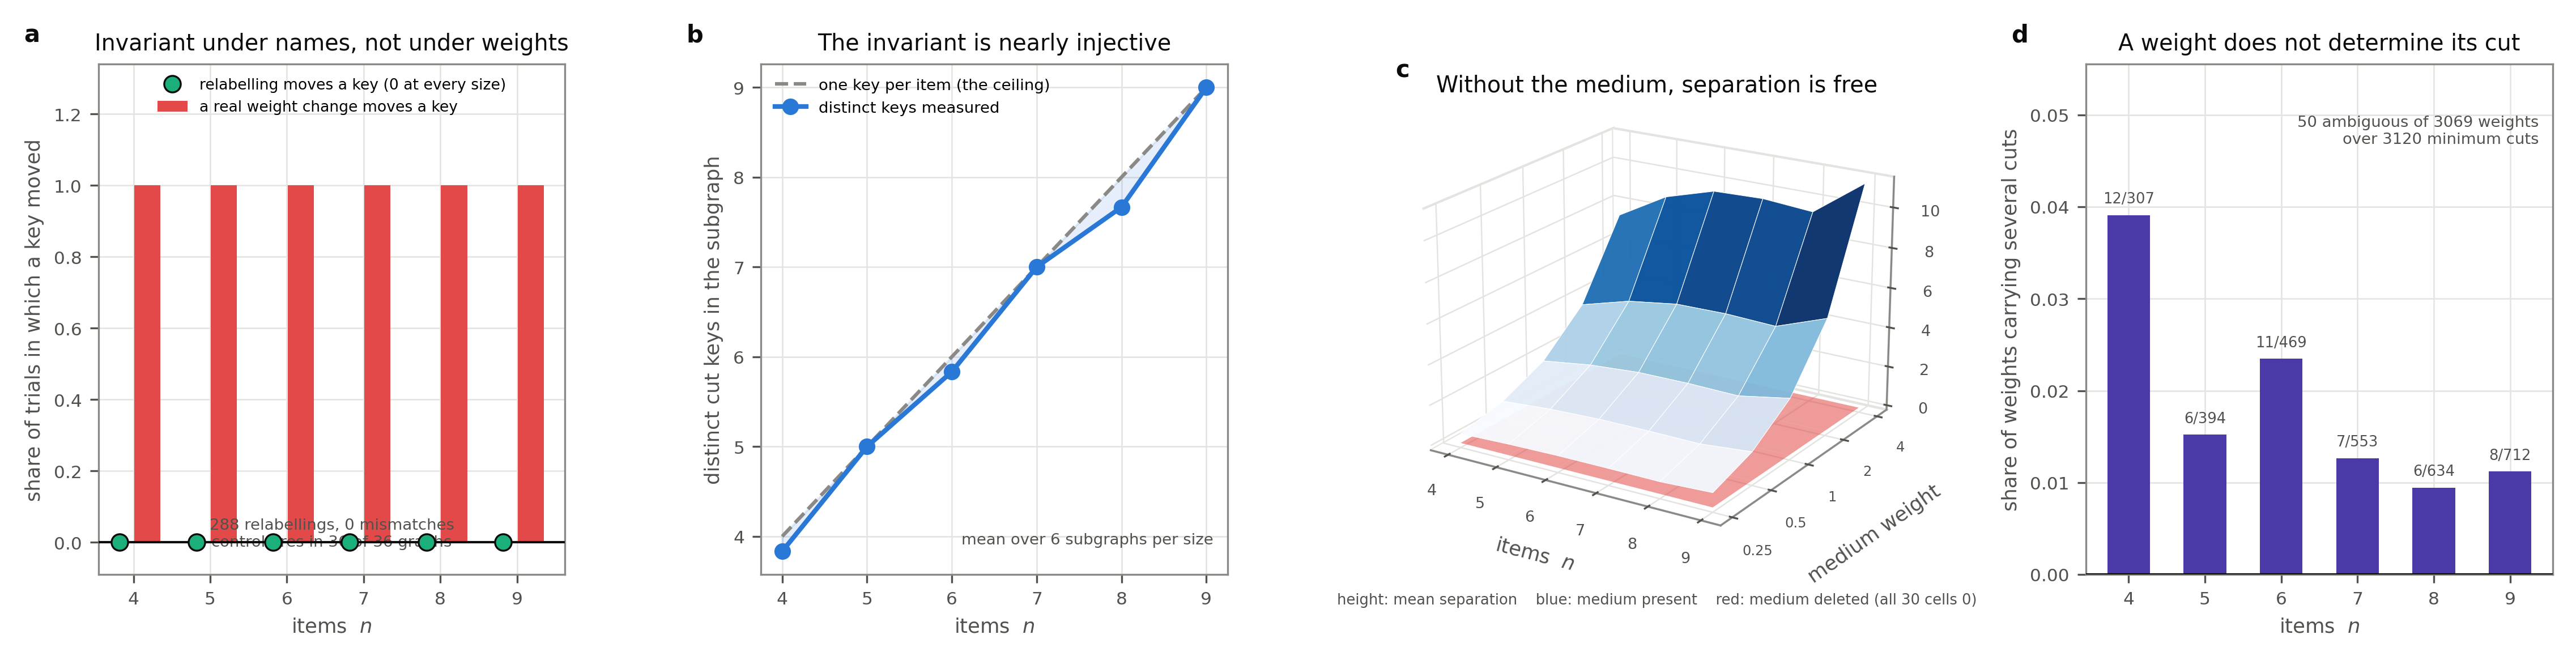
\includegraphics[width=\textwidth]{figures/panel1_invariance.png}
\caption{\Cref{thm:invariance}, \Cref{thm:no-selector} and
\Cref{thm:region} on the NIST library. (a)~relabelling never moves a
key, while a real weight change moves one in every graph.
(b)~distinct keys against items: the invariant is nearly injective.
(c)~mean separation over (items, medium weight), with the medium
present and deleted --- the lower sheet is identically zero in all $30$
cells. (d)~the share of weights carrying several distinct minimum cuts.}
\label{fig:panel-invariance}
\end{figure}

\subsubsection{The key is invariant, and it is not trivial}

\Cref{thm:invariance} was tested by relabelling: $288$ relabellings
across six subgraph sizes moved a key $0$ times. The control fires in
every graph at every size --- scaling one medium edge by $0.25$ moves a
key in $6$ of $6$ graphs at each size --- so this is an invariance claim
rather than a claim that the key is constant.

An invariant that collapses everything to one value is invariant and
useless, so the number of distinct keys was measured against the number
of items. It tracks the item count closely, rising from $3.83$ distinct
keys at $n = 4$ to $9.00$ at $n = 9$: the key separates nearly every
item from every other, which is what makes the invariance worth having.

\Cref{thm:region} was graded against the observation that a scalar
separation could stand in for the separating region --- that is, that
distinct minimum cuts always carry distinct weights. They do not. Over
$3120$ minimum cuts, $50$ of $3069$ weights carry several genuinely
different cuts. The share is a couple of percent and falls with size,
which is why the search had to be powered rather than sampled: at some
sizes a small sample finds none and would report the shortfall as a
refutation.

\subsubsection{Separation is bought entirely from the medium}

\Cref{thm:no-selector} was tested over a grid of five medium weights
and six sizes. With the medium present, separation is positive in all
$12$ graphs at every weight and the minimum separation is at or above
$\flo$ in every cell. With the medium's edges deleted, separation is
\emph{exactly} $0.0$ in all $30$ cells --- not merely cheaper. Deleting
it does not lower the floor, it removes it, and the minimum separation
rises linearly in the medium's weight ($0.2776$, $0.5551$, $1.1103$,
$2.2206$, $4.4412$ at weights $0.25$ through $4$) while remaining flat
in the number of items. This is \Cref{ax:noncomplete} operating rather
than being assumed: the normalisation is what makes any determination
cost anything.

\begin{figure}[htbp]
\centering
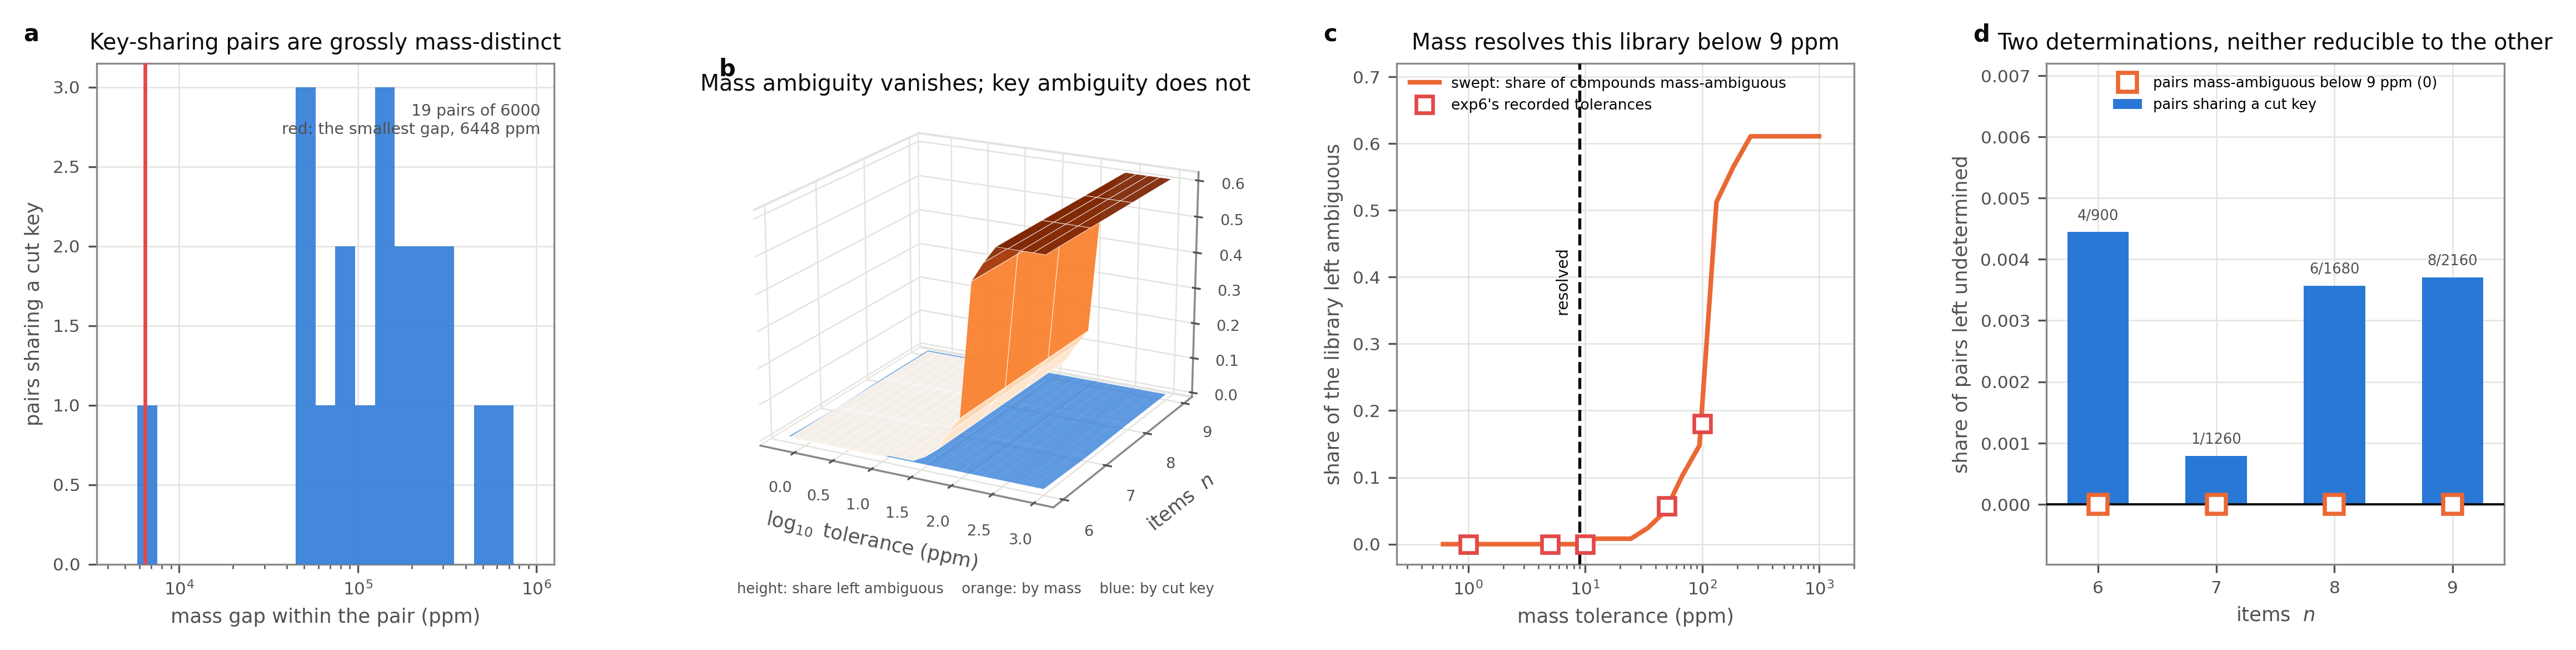
\includegraphics[width=\textwidth]{figures/panel2_mass.png}
\caption{\Cref{cor:mass}. (a)~mass gaps within key-sharing pairs; the
smallest is $6448$ ppm. (b)~ambiguity over (mass tolerance, items) for
each determination: mass ambiguity vanishes with tolerance, key
ambiguity does not. (c)~the library's mass degeneracy against the swept
tolerance, with the recorded points. (d)~the two determinations side by
side per size.}
\label{fig:panel-mass}
\end{figure}

\subsubsection{The key and the mass are independent determinations}

\Cref{cor:mass} says the cut key is not recoverable from the mass, and
the measurement makes the content of that precise. Over $6000$ pairs,
$19$ share a cut key. None of them is near-degenerate in mass: the
\emph{smallest} gap within a key-sharing pair is $6448.2$ ppm, five
orders of magnitude above the tolerance at which the sweep bottoms out.
No refinement of the mass will bring such a pair into agreement, and no
sharpening of the mass will separate them by key.

The honest converse was measured and is recorded rather than suppressed:
mass alone resolves \emph{this} library completely, with $0$ ambiguous
compounds below $9.0$ ppm, and resolution is monotone in the tolerance
over the $23$ points swept. That is a fact about a $244$-compound
library and not a refutation of the corollary. The two are compatible
precisely because the pairs above survive it untouched --- which is what
independence means here, and would be conflated by reporting either
number alone.

\begin{figure}[htbp]
\centering
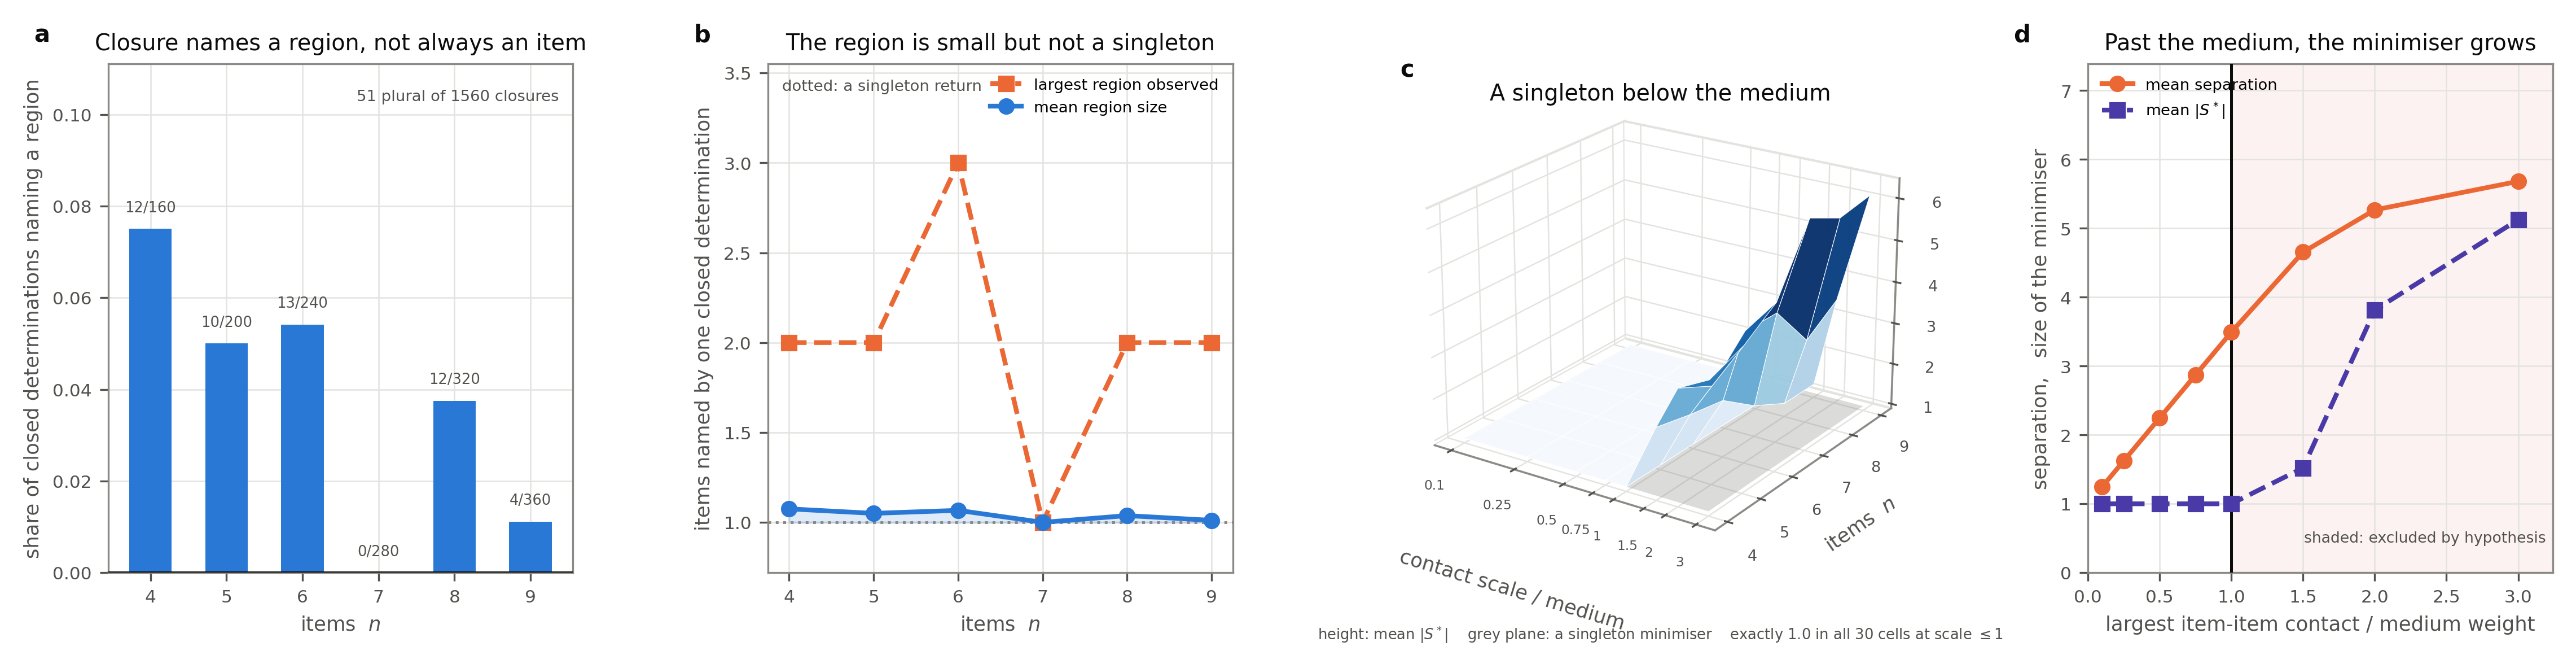
\includegraphics[width=\textwidth]{figures/panel3_closure.png}
\caption{\Cref{def:closure}, \Cref{thm:closure-stronger} and the regime \Cref{ax:noncomplete}
excludes. (a)~the share of closed determinations naming a region rather
than an item. (b)~mean and largest region size. (c)~mean $|S^*|$ over
(contact scale, items): exactly a singleton in all $30$ cells while no
item--item contact exceeds the medium. (d)~the same transition in
section, with the excluded regime shaded.}
\label{fig:panel-closure}
\end{figure}

\subsubsection{Closure names a region, and the regime is what makes it
an item}

\Cref{def:closure} was graded against the observation that a closed
determination always names a single item --- which is the reading
\Cref{thm:closure-stronger}(i) already denies in principle, by
exhibiting a closed determination whose ambiguity set has two
elements. The measurement finds that case at every scale: over
$1560$ closed determinations, $51$ name a plural region, the mean region size
sits just above one at every size, and the largest observed region is
three. Plurality is rare --- a few percent --- and one swept size found
none, which is a sampling gap rather than a structural fact: the mean
region there is exactly $1.0$ over $280$ determinations while both its
neighbours exceed it.

The condition under which closure \emph{does} name an item was then
measured directly, over a grid of six sizes and eight contact scales.
While no item--item contact exceeds the medium, the mean size of the
minimising set is exactly $1.0$ --- to machine precision, in all $30$
cells at scale $\le 1$, at every size. Past the medium the floor breaks
and the minimiser grows with the number of items, reaching $5.125$ at
scale $3$. This is what \Cref{ax:noncomplete}'s normalisation buys and
it is the regime the axiom excludes by hypothesis; the measurement shows
the exclusion is doing work rather than being a convenience.

\begin{figure}[htbp]
\centering
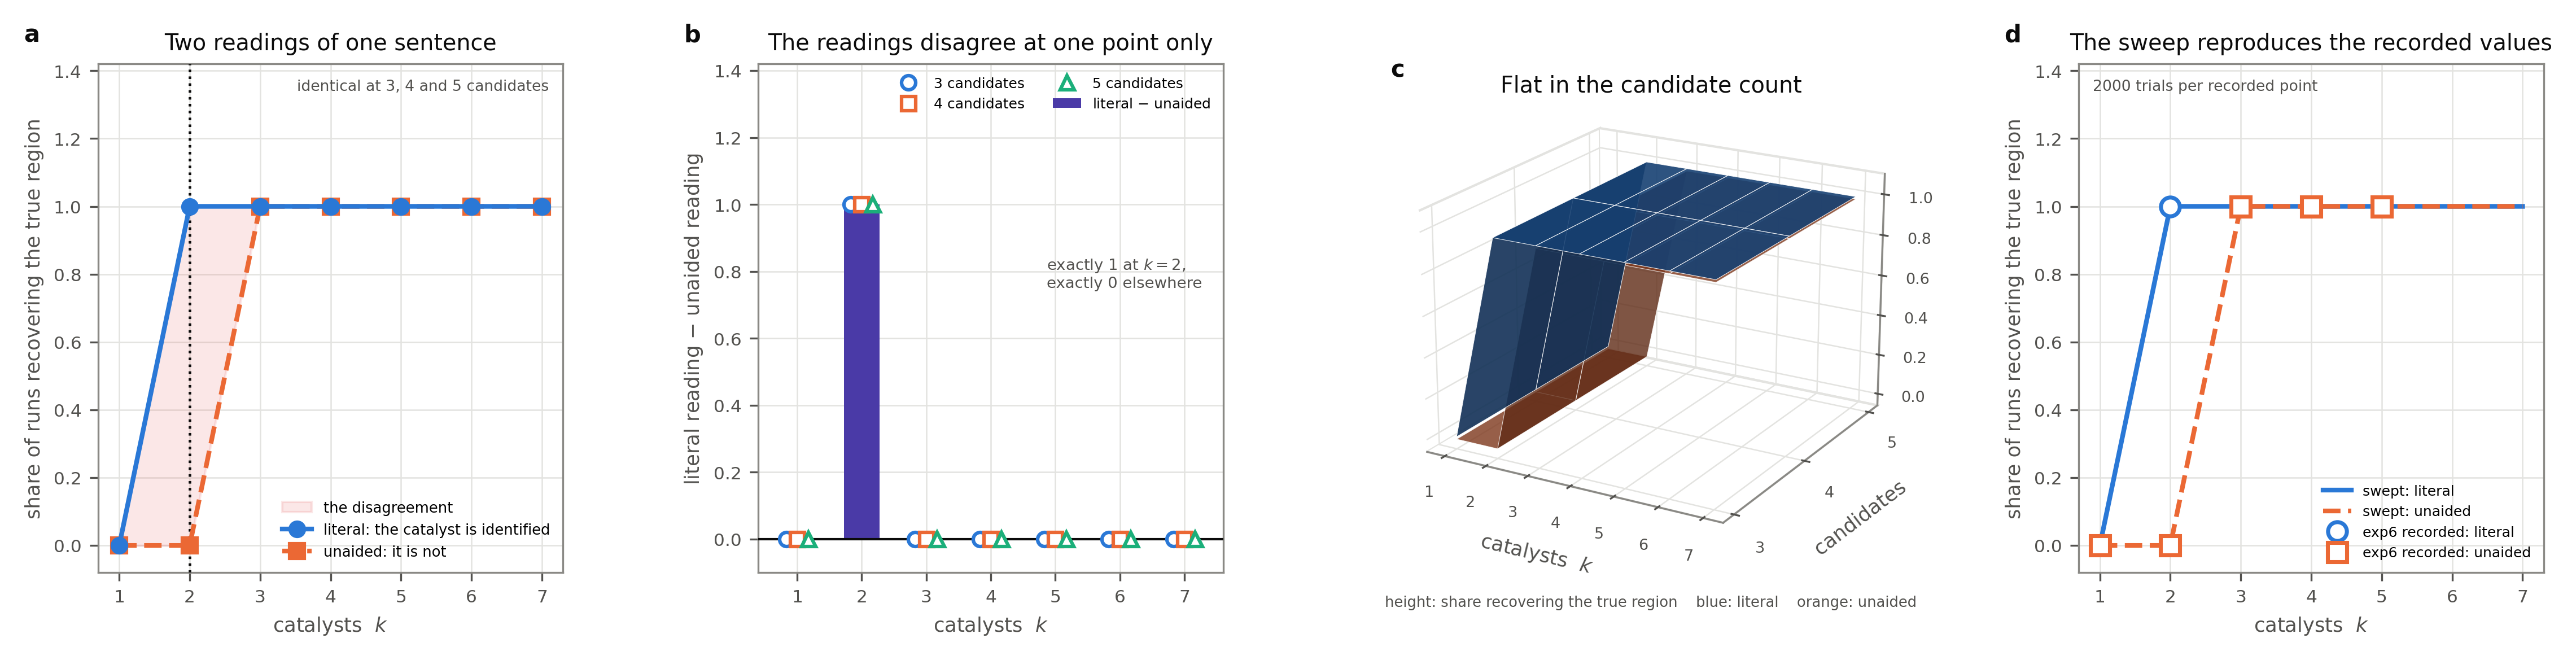
\includegraphics[width=\textwidth]{figures/panel4_three.png}
\caption{\Cref{prop:three}, which the suite did not reproduce.
(a)~the two readings of the proposition against $k$; they differ at
$k = 2$ and nowhere else. (b)~the gap between the readings, exactly $1$
at $k = 2$ and exactly $0$ elsewhere, at each candidate count.
(c)~both readings over $(k, \text{candidates})$: flat in the candidate
count. (d)~the swept curves against the recorded points.}
\label{fig:panel-three}
\end{figure}

\subsubsection{A defect in the statement of
\texorpdfstring{\Cref{prop:three}}{Proposition: three catalysts}}
\label{ssec:three-defect}

\Cref{prop:three} did not reproduce, and the measurement locates the
fault precisely enough to say what should be changed.

The proposition's wording admits two incompatible readings. Read
literally, \emph{``the erroneous catalyst''} is definite: it is
identified, removed, and the majority taken over the survivors. Under
that reading $k = 2$ already suffices --- measured at $1.000$ of runs
recovering the true region. Read as the proof's reason describes it, the
erroneous catalyst is \emph{not} identified and the majority runs over
all $k$; under that reading $k = 2$ recovers the true region in $0.000$
of runs and $k \ge 3$ is required, which is what the proposition
asserts.

The two readings agree at every $k$ except $k = 2$, where they differ by
exactly one. That single point is the whole of the disagreement, and it
is identical at $3$, $4$ and $5$ candidates, so it is not an artefact of
the candidate pool. Each recorded point rests on $2000$ trials, and the
swept curves pass through exactly the values the experiment recorded.

The defect is therefore in the statement, not the proof: the reason
given is sound for the unaided case, and the definite article claims
more than that case supports. The proposition should read \emph{``an
erroneous catalyst''} and state explicitly that the erroneous one is not
identified. With that amendment the bound $k \ge 3$ is correct and tight
--- at $k = 3$ both readings recover the true region in $1.000$ of runs.
We report it as not reproduced rather than silently repairing it,
consistent with the treatment of \Cref{ass:structure} above.

\subsubsection{What this second suite does not establish}

The library is $244$ formulae, and the mass-resolution result is a
property of that library rather than of libraries in general; a denser
one would resolve at a sharper tolerance and the corollary would be
unaffected either way, since the key-sharing pairs are mass-distinct by
four orders of magnitude. The graph claims are exercised on subgraphs of
between four and nine items, which is what permits exhaustive
minimisation over cuts; the cost claims are not tested at scale here.
\Cref{ax:noncomplete} is imposed rather than tested --- what is measured
is the difference between the regime it admits and the regime it
excludes, which is a singleton minimiser against one that grows.

% =====================================================================
\section{Limitations}
\label{sec:limitations}
% =====================================================================

\paragraph{The promiscuity claim is withdrawn.} \Cref{ass:structure}
carried the empirical claim of \Cref{sec:promiscuity} and is refuted in
\Cref{sec:validation}, with the departure from independence running
opposite to the predicted direction. Expectation E5 fails and its
negative control N1 fails to fail. We have not repaired the claim by
weakening it: it is reported as refuted, the development is retained
because the refutation is instructive, and readers should treat
\Cref{sec:promiscuity} as an account of why shared peptides are usable
rather than as a recommendation to prefer them. The remaining theorems
do not depend on it.

\paragraph{The statement of \Cref{prop:three} is defective.} The
proposition did not reproduce, and \Cref{ssec:three-defect} locates the
fault in its wording rather than in its proof. \emph{``The erroneous
catalyst''} is definite, and read that way $k=2$ suffices; the reason
the proof gives describes the case in which the erroneous catalyst is
not identified, where $k\ge3$ is required. The two readings differ at
$k=2$ and nowhere else, identically at three, four and five candidates.
The bound is correct under the intended reading and the statement should
be amended to \emph{``an erroneous catalyst''}, made explicit that it is
unidentified. We report it as not reproduced rather than silently
repairing it.

\paragraph{Synthetic proteome.} The proteome-level validation uses a
generated proteome with domain-based sharing, not a measured one; only
the graph and mass claims of \Cref{ssec:three-defect} and the
subsections preceding it were exercised on measured data. It was built to have the
structure the assumption named, and the assumption still failed, which
is the strongest form the negative result could take on this data; but a
real proteome may depart in further ways, and no claim here is
established on measured biological sequence.

\paragraph{The framework is not a spectrum interpreter.} It says when a
determination may stop and what it returns. It does not pick peaks,
deisotope, compute fragment intensities, or compete with an established
search engine on identification rate. A complete system requires both.

\paragraph{Cut keys are invariants, not canonical forms.} $\key$ does not
totally order items and cannot serve directly as a canonical labelling.
Iterated refinement inherits the known incompleteness of colour
refinement on strongly regular
graphs~\citep{weisfeiler1968,cai1992optimal}.

\paragraph{Weights are modelling choices.} \Cref{tab:edges} lists edge
classes but not a principled scale for their weights. Different weightings
give different residuals. The theorems are weight-independent; the
numerical results are not.

\paragraph{The floor is not measured.} $\flo$ is derived to be positive
and computed within a given graph, but the framework provides no
absolute scale for it, and no experiment here determines a physical
value.

\paragraph{Closure is relative to available catalysts.} A determination
closed under one set of methods may reopen when a new method becomes
available. This is a feature---it is how the periodic table was
populated---but it means closure is not permanence.

% =====================================================================
\section{Conclusion}
\label{sec:conclusion}
% =====================================================================

A mass spectrometer of unbounded resolution cannot identify lithium
because identity is a region and a mass is a point. The periodic table's
cell for lithium is the terminus of a sufficient not-lithium sequence,
and the array of instruments chemistry brings to bear on one element is
not redundancy but necessity: each commits a different exclusion, and
none individuates alone.

Carried to peptides, this yields three results that survive measurement.
Identity is the invariant minimum cut, region-valued and bounded below by
a floor (\Cref{thm:region}). Edges redistribute residual rather than
accumulating knowledge, so what an analysis measures is what remains
unknown (\Cref{thm:residual}). And a determination terminates at
closure---when further evidence stops moving the claim region---which is
strictly stronger than a confidence threshold and yields a two-outcome
dichotomy with a computable bound (\Cref{thm:closure-stronger},
\Cref{thm:dichotomy}). All three were checked numerically and hold.

A fourth claim did not survive. We proposed that protein inference should
rank peptides by how much they exclude rather than by how few proteins
they implicate, and registered the expectation before testing it. It is
false. \Cref{thm:collapse} is monotone increasing in each promiscuity, so
its own arithmetic favours the least promiscuous peptide; the
uniqueness-first control that was designed to fail instead won every
trial; and the supporting assumption about proteome structure is refuted
with the opposite sign. What remains true is the weaker and still useful
statement that shared peptides carry multiplicative discriminating power
in combination and should not be discarded---not that they should be
preferred.

Two consequences are worth stating plainly. An isobaric pair such as
$\{L,I\}$ is a correct closed answer under mass evidence rather than a
failure to resolve; and a spectrum whose exclusion sequence has not
closed is not an unidentified spectrum but a located deficiency in the
evidence, which \Cref{prop:disagree} attributes either to the reference
set or to the preparation chain. The unannotated fraction of a typical
experiment~\citep{michalski2011more} is, on this account, not noise but
peptides whose not-$X$ sequences have not yet terminated.

\bibliographystyle{plainnat}
\bibliography{references}

\end{document}
